\section{Query Languages}
\label{sec:querymod}

In a DSPS, data is continuously pushed into the system in the form of streams. These are real-time,
continuous, ordered sequences of data items. Streams have different characteristics than traditional
relations in a DBMS, and the way of expressing queries in a DSPS has to take these differences into
account. Streams can be unbounded but queries are usually issued over a recent snapshot of the data
stream, which is referred to as \textit{window}. A query language for data streams must be capable of
operating over windows of data, should be extensible in order to support custom user operators, and
simple enough to enable the easy specification of complex queries. 

Three query paradigms have been proposed for streaming data~\cite{dsm-issues}. The first and
most adopted is the \textit{relational streaming model}. It comes from the DBMS world and is
usually implemented as an SQL-like language. It provides the syntax to express windows over data streams,
similarly to the extensions introduced in SQL-99. A query describes the results in a declarative way,
giving the system the flexibility of selecting an optimal evaluation procedure for producing the desired
answer. Examples of languages employing this model are CQL~\cite{cql}, StreamSQL~\cite{streamsql} and
SPACE~\cite{ss-spade}. 

Another method for expressing queries is through \textit{procedural streaming languages}. In this
paradigm, the user constructs queries in a graphical way, having maximum control over the exact series of
steps by which the query answer is obtained. In this model, operators are depicted as boxes and arrows
represent the data streams flowing through them, thus taking the name of \textit{boxes-and-arrows} model.
One drawback of this model is the difficulty of expressing complex query plans because the diagram
describing a query can become intricate. Aurora~\cite{aurora} and Borealis~\cite{borealis-design} are
examples of systems employing this query model.

The third model for expressing queries is the \textit{object-oriented streaming paradigm}. In this
approach, the query elements are modeled in a hierarchical way, taking inspiration from the
object-oriented programming world. In Cougar~\cite{cougar-adt}, for example, sources are modeled as ADTs
(Abstract Data Types), exposing an interface consisting of a sensor's signal processing methods. A discussion of
query languages and practical issues on building a stream processing system can be found
in~\cite{design-principles}.

The next sections present more details on the two main models for expressing queries in a
stream processing system: the \emph{continuous query language} and the \emph{boxes-and-arrows}
representation.

\subsection*{CQL: Continuous Query Language}
\label{sec:cql}

The Continuous Query Language~\cite{cql} is a declarative language for expressing continuous queries
over streams of data. It has been introduced as part of STREAM (Stanford Stream Data
Manager)~\cite{stream} and has become one of the de facto standards in stream processing. It is an
SQL-like language designed to work on streams as well as with relations and to allow an easy conversion
among them. It extends SQL, introducing semantics to enable queries to be issued over streams of data. A detailed description of the
more formal aspects of the language can be found in~\cite{cql-foundation}. 

To better illustrate the main concepts in CQL, let us consider a \textit{temperature monitoring} query.
The purpose of such a query is to detect if the temperature in any room of a building rises above a
certain threshold. If a room becomes too hot, the system detects it and reacts by switching on the local
air conditioning unit. In this scenario, all rooms are equipped with thermal sensors.
These are connected to a stream processing system, which is able to control the air conditioning unit.
The thermal sensors sample the temperature in the room every minute, sending these readings, together with
their room id and timestamp, to the stream processing system. This executes a simple query, filtering
all tuples with a temperature reading above a certain threshold (\eg $T>=30$). When the system
detects that a room is too hot, it switches on the air conditioning unit in that room. 
\subsubsection*{Data Types}

The two core data types manipulated by CQL are \textit{streams} and \textit{relations}.

\begin{definition}[Stream]{A stream S is a potentially infinite bag (multiset) of elements $\langle s,
\tau \rangle$, where $s$ is a tuple belonging to the schema of $S$ and $τ ∈ T$ is the timestamp of the element.}
\end{definition}

Timestamps are not part of the schema of a stream, and there can be zero, one or more elements with
a given timestamp in a stream. The number of elements with the same timestamp in a stream is finite but
unbounded.
In CQL the data part of a stream element is referred to as a \textit{tuple}. There are
two classes of streams: \textit{base streams}, which are the input of the system, and \textit{derived
streams}, which are intermediate streams produced by operators. 

\underline{\textsc{Example}}: In our temperature monitoring scenario there would be only one base stream
with a schema: \textsc{RoomTmpStr(RoomID, RoomTmp)}. Attribute \textsc{RoomID} identifies the room where
the sensor is located, while \textsc{RoomTmp} contains the current detected temperature. 

\begin{definition}[Relation]{A relation R is a mapping from each time instant T to a finite but
unbounded bag (multiset) of tuples belonging to the schema of R.}
\end{definition}

A relation $R$ defines an unordered multi-set of tuples at any instant in time $\tau \in T$,
denoted as $R(\tau)$. The difference between this definition and the one used in databases is that, in
the standard relational model, a relation is simply a set of tuples with no notion of time. 

\underline{\textsc{Example}}: In our scenario, a relation is created from the base stream of
temperature readings through a time-window operator. It is a snapshot of all readings received within the last
minute. The concept of windows over streams will be explained in the next paragraph.

\subsubsection*{Operator Classes}
\begin{figure}[b]
	\centering
	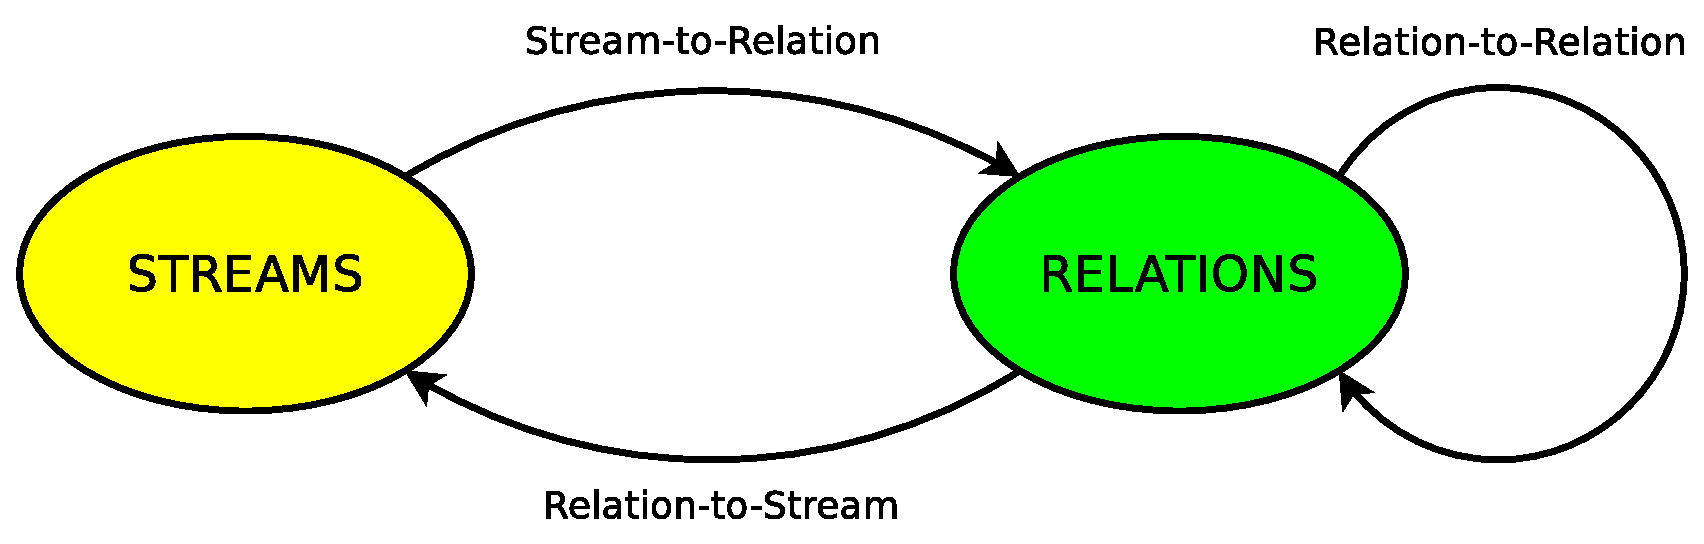
\includegraphics[width=0.8\textwidth]{img/tesi/cql_ops} 
	\caption{Interaction among the three classes of operators in CQL.}
	\label{fig:cql_ops}
\end{figure}
CQL employs three classes of operators to process stream data. First is the \textit{Stream-to-Relation}
operator, which creates a snapshot of a stream. After a finite bag of tuples has been
obtained, it employs \textit{Relation-to-Stream} operators, which are equivalent to the ones employed in
a traditional DBMS. Finally, there are \textit{Relation-to-Stream} operators to create streams from
newly computed relations. Figure~\ref{fig:cql_ops} shows the interaction between these classes of
operators. 

\paragraph{Stream-To-Relation} operators are used to isolate a subset of a stream, or snapshot, so that
one or more relation-to-relation operators can act on it. All the operators in this class are based on
the concept of a \textit{sliding window} over a stream. This contains, at any point in time, a
historical snapshot of a finite portion of the stream. 

Three kinds of window operators exist in CQL: time-based, tuple-based and partitioned. A
\textit{time-based} window contains all the tuples in the stream that have timestamps within the
specified boundaries. For example, it could hold all the tuples that have arrived in the past minute. In
a \textit{tuple-based} window, instead, the number of tuples is specified and fixed so that it only
contains the last $N$ tuples of the stream. A \textit{partitioned} window is a special kind of the
tuple-based window. It allows the user to specify a set of attributes as a parameter, splits the
original stream based on these arguments, similarly to the SQL GroupBy statement, and computes a
tuple-based window of size $N$ independently creating a number of substreams.

\textit{Sliding Windows} produce a snapshot of a stream based on two parameters: the \textit{window size}
and the \textit{sliding factor}. Once the window is triggered, it outputs all the tuples that it
contains but it does not discard them all. The sliding factor determines a strategy to hold some tuples
in the window so that they can be used in the next iteration. A tuple-based window, for example, can be
set to trigger every 5~tuples with a slide of 1. Every time that it reaches 5 tuples, it outputs all of
them but retains the 4~most recent tuples for the next iteration. A time-based window can be set to
trigger every five minutes with a sliding factor of 1~minute. At every iteration, it outputs all the
tuples that have arrived in the past 5 minutes, retaining all tuples from the past 4 minutes. 

\paragraph{Relation-To-Relation} operators are derived from the traditional SQL relational model. They
perform the bulk of the data manipulation and are equivalent to canonical SQL operators. In this
category, we find, for example, \textsc{Select, Project} and other familiar operators. A stream is
converted into a relation by a window operator, then processed by a relation-to-relation operator and finally output by
a relation-to-stream operator.
			
\underline{\textsc{Example}}: Consider the following query for our temperature monitoring scenario:

\tab \textsc{Select *} \\
\tab \textsc{From RoomTmpStr[Range 5 Min]} \\
\tab \textsc{Where Tmp > 30} 

This query is composed of a stream-to-relation time-window operator, followed by a relation-to-relation
operator performing a projection. The output is a relation that contains, at any time, the set of all
temperature readings received by the system in the past five minutes with temperatures greater than 30
degrees Celsius. 

\paragraph{Relation-To-Stream} operators convert the result of relation-to-stream operators back into a
stream. Three kinds of such operators exists in CQL: \textit{IStream, DStream} and \textit{RStream}.

1. \textbf{IStream} (for ``insert stream'') outputs only the new tuples that have been generated since
the last execution. It compares the current output of the preceding relation-to-relation operator and
outputs all the tuples that are present in the current input but not in the previous one. Informally, it
inserts new tuples into the stream. Formally, the output of \textit{IStream} applied to a relation $R$
contains a stream element $\langle s, \tau \rangle$ whenever tuple $s$ is in $R(\tau)-R(\tau-1)$. Assuming
$R(-1)=\emptyset$, we have: %XXX: fix parentesis

\begin{center}
	$IStream(R) = \bigcup_{\tau>=0}\Big[(R(\tau)-R(\tau-1))\times\{\tau\}\Big]$ %fix union
\end{center}

2. \textbf{DStream} (for ``delete stream'') outputs only tuples that have disappeared since the last
execution. It compares the current output of the preceding relation-to-relation operator and
outputs all the tuples that were present in the previous input but not in the current one. Informally,
it generates the stream of tuples that have been deleted from the relation. Formally, the output of
\textit{DStream} applied to a relation $R$ contains a stream element $\langle s, \tau \rangle$ whenever tuple $s$ is in
$R(\tau-1)-R(\tau)$. %XXX: fix parentesis

\begin{center}
	$DStream(R) = \bigcup_{\tau>=0}\Big[(R(\tau-1)-R(\tau))\times\{\tau\}\Big]$ %fix union
\end{center}

3. \textbf{RStream} (for ``relation stream'') informally outputs all tuples produced by the
relation-to-relation operator. Formally, the output of \textit{RStream} applied to a relation $R$
contains a stream element $\langle s, \tau \rangle$ whenever tuple $s$ is in $R$ at time $\tau$.

\begin{center}
	$RStream(R) = \bigcup_{\tau>=0}\Big[(R(\tau)\times\{\tau\}\Big]$ %fix union
\end{center}	

\begin{figure}[b]
	\centering
	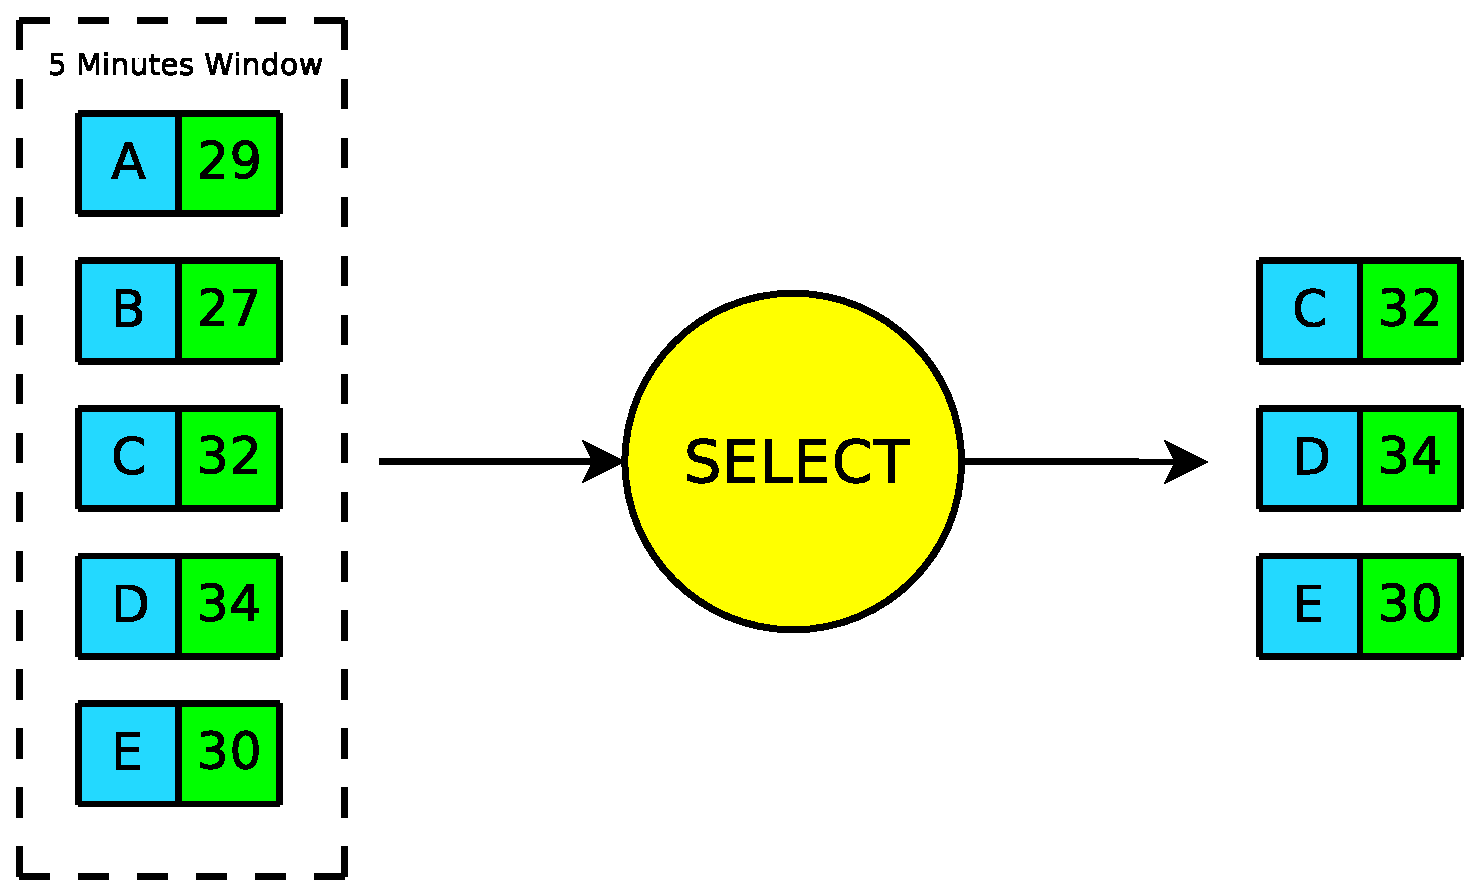
\includegraphics[width=0.55\textwidth]{img/tesi/cql-example} %XXX: rifare figura
	\caption{This query outputs all tuples with a temperature reading $\geq$ 30 in the last five minutes.}
	\label{fig:cql-example}
\end{figure}
\vspace{15pt}
\underline{\textsc{Example}}: Figure~\ref{fig:cql-example} illustrates a simple CQL query implementing
our temperature monitoring scenario. It signals all rooms, in which a temperature above 30~degrees
Celsius is detected in the past 5~minutes. The input stream is called \textsc{RoomTmpStr} and carries
tuples formed by a room identifier (\textsc{RoomId}) and a temperature reading (\textsc{RoomTmp}). A time-based window
is applied to it to obtain a snapshot that contains only fresh measurements generated in the past five
minutes. Once this relation has been created, a conditional \textsc{Select} is used to filter
out all tuples with a temperature value lower than 30~degrees. Finally, a new stream called
\textsc{HotRoomsStr} is created by an \textsc{IStream} relation-to-stream operator, containing tuples
from overheated rooms, which are then sent to control the air conditioning subsystem.
\vspace{15pt}

\tab \textsc{Select IStream(*)} \\
\tab \textsc{From RoomTmpStr[Range 5 Min]} \\
\tab \textsc{Where Tmp > 30} \\

\clearpage
%BOXES AND ARROWS
\subsection*{Boxes-and-Arrows Model}
\label{boxes_and_arrows}
A different paradigm to express queries over streams is the
\emph{boxes-and-arrows} model~\cite{boxes-and-arrows}.
It was introduced as part of the project Aurora~\cite{aurora-and-medusa} and also employed by
Borealis~\cite{borealis-design}.
In this model, a query is represented graphically as a data flow graph. Operators are depicted as boxes,
with streams being arrows connecting them. Tuples flow in a loop-free, directed graph of processing
operations. Queries in this model are specified by composing the query plan using a graphical interface
or by employing a query language such as SQuAl (Stream Query Algebra).
Aurora employs its own set of primitive operators, even though many of these have equivalents in a
traditional relational query model.
In this model, we can divide operators into two main categories: stateless and
stateful~\cite{borealis-app-manual}.

\paragraph{Stateless operators.} Steteless operators do not need to store any information about previous
tuples in order to execute.
\emph{Map} is an example of such an operator. It transforms some attributes of a tuple by applying a
predicate. If we consider a tuple carrying a temperature reading, for example, a Map operator can be
used to convert the temperature field from degrees Fahrenheit to Celsius.\\
In the same category, there is also a \emph{Filter} operator. It can be seen as the equivalent of a
\emph{Select} in the relational model.
It applies predicates to each input tuple and includes them in an output stream if the predicate evaluates to \emph{true}.
A Filter operator can have multiple output streams, depending on the number of specified predicates. \\
\emph{Union} is a simple operator that produces a single output stream from many input streams with the
same schema. The operator itself does not modify the tuples but it simply merges
streams. For example, it is used to provide a single stream as an input to other
operators, such as an Aggregate or a Filter.

\paragraph{Stateful operators.} Stateful operators maintain internal state, which is determined by the
tuples processed previously. 
In the boxes-and-arrows model, there is no explicit concept of a \emph{window} operator, unlike in CQL.
Instead, some operators are designed to support windowing on their input streams. The semantics for
expressing these windows are rich, and it is possible to state a wide range of windows, such as
count-based, time-based and partitioned. A sliding parameter can be used to specify the updating policy
of the window.\\
\emph{Aggregate} is a typical example of such an operator. It computes an aggregate function, such as a
sum or an average, over a window of tuples. A wide range of aggregate functions is provided, and others
can be specified by the user. It accepts a single input stream and is usually preceded by a Union operator. 
\emph{Join} is another classical stateful operator with two input streams and two windows. Join pairs
tuples from the two input windows that satisfy a given predicate, resembling its
relational~counterpart.\\
A special kind of stateful operators are synchronisation operators. This class includes \emph{Lock,
Unlock} and \emph{WaitFor}. These are used to buffer tuples temporarily until a certain condition is
reached.

\paragraph{\mbox{Load-shedding} operators.} Load-shedding operators are used to overcome overload
conditions. They reduce the load of an operator by discarding a portion of its input. This category includes RandomDrop and
WindowDrop. \emph{RandomDrop} randomly discards a certain fraction of a stream. Every time the operator
is scheduled, it discards a number of tuples on its input window at random according to specified
dropping parameters. \emph{WindowDrop} allows for a more sophisticated specification of the windowing
parameters. Once a window has been computed, it choose probabilistically if it should be kept or
discarded as a whole according to a dropping parameter.\\

% In Borealis, some other operators have been introduced to deal with fault-tolerance~\cite{revision-processing}. 
% As better described in Section~\ref{sec:borealis}, Borealis aims at eventual consistency, meaning that, once the system has recovered from failure, 
% it will try to replay some tuples and eventually correct its previously tentative results. \emph{RevisionJoin, RevisionAggregate} and \emph{RevisionFilter} are examples of operators used for this operations. Furthermore, replication can be employed to improve the dependability of the system. This means that
% some subsets of the query plan, called replica sets, are run in parallel at different sites, so that if a crash should happen at the processing node hosting a set of replicated operators, the system can continue to operate using the output of another replica set. When working with replication, some of the operators have to be substituted by their deterministic version, which only forward tuples coming from one replica set, usually the first ones to arrive. These operators have the same name as their traditional counterparts, with the difference of an initial $S$, for instance \emph{SUnion, SFilter} and \emph{SJoin}. 
% When employing these operators, replicas are actively competing to deliver results as soon as possible, improving non only enhancing the availability of the system but also improving its performance in terms of end-to-end latency~\cite{borealis-fast_and_reliable, borealis-fast_and_ha}.

\underline{Example:}\\
In the boxes-and-arrows model, implementing our temperature monitoring query is simple. 
Figure~\ref{fig:baa-example} shows the graphical representation of this query.
In this case, the query plan is composed only of a \emph{Filter} operator. It receives the stream of 
readings as input and outputs all tuples satisfying the predicate T $\geq$ 30. 

\begin{figure}[t]
    \centering
    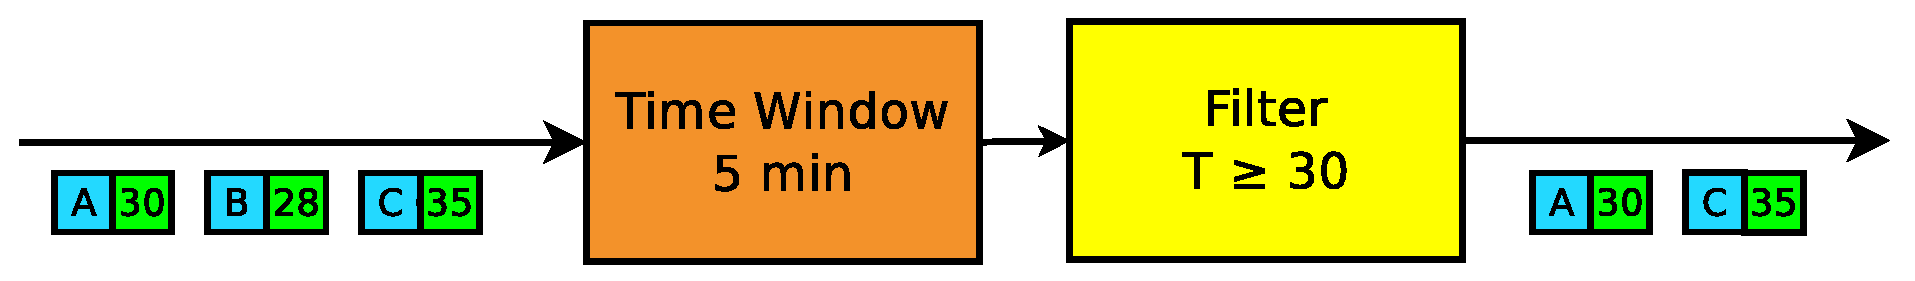
\includegraphics[width=0.8\textwidth]{img/tesi/baa-example}
    \caption{Temperature monitoring query example, expressed in the boxes-and-arrows model.}
    \label{fig:baa-example}
\end{figure}